\documentclass{amsart}

\usepackage{amsmath}
\usepackage{amssymb}
\usepackage{amsfonts}
\usepackage{geometry}
\usepackage{graphicx}
\usepackage{amsmath,amssymb,amsthm}
\usepackage{mathtools}
\usepackage{tikz}
\usetikzlibrary{calc,angles,quotes,decorations.markings,arrows.meta,shapes.geometric,positioning,fit,backgrounds,patterns}
\usepackage{xcolor}
\usepackage{microtype}
\usepackage{hyperref}
\usepackage{listings}
\usepackage{caption}


\lstset{
	language=Matlab,
	basicstyle=\ttfamily\footnotesize,
	keywordstyle=\color{blue},
	stringstyle=\color{morleypurple},
	commentstyle=\color{morleygreen},
	numbers=left,
	numberstyle=\tiny\color{gray},
	stepnumber=1,
	numbersep=8pt,
	breaklines=true,
	frame=single,
	rulecolor=\color{gray!40},
	backgroundcolor=\color{morleylight!50},
	showstringspaces=false,
	captionpos=b,
	aboveskip=1.5em
}

\definecolor{morleydark}{RGB}{45,35,55}
\definecolor{morleymain}{RGB}{120,80,140}
\definecolor{morleyaccent}{RGB}{200,140,80}
\definecolor{morleylight}{RGB}{245,240,235}
\definecolor{morleygold}{RGB}{190,150,70}
\definecolor{morleyblue}{RGB}{75,100,150}
\definecolor{morleygreen}{RGB}{85,130,95}
\definecolor{morleyred}{RGB}{155,75,75}
\definecolor{morleypurple}{RGB}{130,90,140}

\geometry{a4paper, margin=1in}

\newtheorem{theorem}{Theorem}[section]
\newtheorem{lemma}[theorem]{Lemma}

\makeatletter
\def\@tocline#1#2#3#4#5#6#7{\relax
	\ifnum #1>\c@tocdepth % then omit
	\else
	\par \addpenalty\@secpenalty\addvspace{#2}%
	\begingroup \hyphenpenalty\@M
	\@ifempty{#4}{%
		\@tempdima\csname r@tocindent\number#1\endcsname\relax
	}{%
		\@tempdima#4\relax
	}%
	\parindent\z@ \leftskip#3\relax \advance\leftskip\@tempdima\relax
	\rightskip\@pnumwidth plus4em \parfillskip-\@pnumwidth
	#5\leavevmode\hskip-\@tempdima
	\ifcase #1
	\or\or \hskip 1em \or \hskip 2em \else \hskip 3em \fi%
	#6\nobreak\relax
	\dotfill\hbox to\@pnumwidth{\@tocpagenum{#7}}\par
	\nobreak
	\endgroup
	\fi}
\makeatother

\renewcommand{\contentsname}{\centering \Large TABLE OF CONTENTS}

\begin{document}
	
	% ==========================================
	% SHEET 1: TITLE PAGE
	% ==========================================
	\begin{titlepage}
		\centering
		\vspace*{1.5cm}
		
		{\Large{Morley's Trisector Theorem: A Multi-perspective approach}\par}    
		\vspace{1.2cm}
		
		{\normalsize{A Report}\par}
		\vspace{1.2cm}
		
		{\normalsize\itshape
			Submitted in partial fulfilment of the requirements for \textit{course}\par}
		\vspace{1.5cm}
		
		{\large{MAC-291}\par}
		\vspace{1.2cm}
		
		{\normalsize\itshape in\par}
		\vspace{1.2cm}
		
		{\large{Mathematics}\par}
		\vspace{1.2cm}
		
		{\normalsize\itshape by\par}
		\vspace{1.2cm}
		
		{\large{Sanatan Kumar Gupta }\par}                
		{\normalsize (Enrol.\ No.\ 24323035)\par} 
		\vspace{2cm}
		
		\includegraphics[width=0.1\textwidth]{iitr_logo} 
		\vspace{1.2cm}
		
		{\large{Indian Institute of Technology Roorkee}\\[0.2em]
			{April 19, 2026}\par}
	\end{titlepage}
	
	% ==========================================
	% SHEET 2: CERTIFICATE
	% ==========================================
	\newpage
	\thispagestyle{empty} 
	\vspace*{1.5cm}
	
	\begin{center}
		\Large \textbf{CERTIFICATE}
	\end{center}
	\vspace{1.5cm}
	
	\begin{center}
		\textbf{Student's Declaration}
	\end{center}
	\vspace{0.5cm}
	
	\noindent I hereby certify that the work presented in this report titled ``\textbf{Morley's Trisector Theorem: A Multi-perspective approach}'' is carried out by me. This is a new presentation of a work existing in the literature. The contents that are taken from the literature are cited properly by providing the best possible reference. It is further certified that the use of AI is limited to simulation and analysis of data. All the other contents were prepared by me.
	
	\vspace{1.5cm}
	\noindent
	\begin{minipage}{0.5\textwidth}
		\textbf{Date: 19th April, 2026}
	\end{minipage}%
	\begin{minipage}{0.5\textwidth}
		\raggedleft
		\includegraphics[width=.2\textwidth]{sign.jpg} \\
		\textbf{Signature} 
	\end{minipage}
	
	\vspace{2.5cm}
	
	\begin{center}
		\textbf{Supervisor's Declaration}
	\end{center}
	\vspace{0.5cm}
	
	\noindent This is to certify that the above mentioned work is carried out under my supervision.
	
	\vspace{1.5cm}
	\noindent
	\begin{minipage}{0.5\textwidth}
		\textbf{Date:} \rule{3cm}{0.4pt}
	\end{minipage}%
	\begin{minipage}{0.5\textwidth}
		\raggedleft
		\textbf{Signature:} \rule{4cm}{0.4pt}
	\end{minipage}
	
	% ==========================================
	% ABSTRACT PAGE
	% ==========================================
	\newpage
	\pagenumbering{roman} 
	
	\begin{center}
		\Large \textbf{ABSTRACT}
	\end{center}
	\vspace{1cm}
	Morley's Trisector Theorem is a fundamental result in elementary geometry stating that the three points of intersection of the adjacent trisectors of any triangle's angles form an equilateral triangle. Discovered by Frank Morley in 1899, the theorem has since received multiple independent proofs. This report presents five proofs drawn from different mathematical domains (trigonometry, complex-number algebra, synthetic geometry, group theory, and circle geometry).
	
	% ==========================================
	% TABLE OF CONTENTS & LIST OF FIGURES
	% ==========================================
	\newpage
	\addtocontents{toc}{\noindent \textbf{CHAPTER NO.} \hfill \textbf{TITLE} \hfill \textbf{PAGE NO.}\par}
	\addtocontents{toc}{\noindent \rule{\textwidth}{0.5pt}\par\vspace{0.2cm}}
	\tableofcontents
	
	\newpage
	\renewcommand{\listfigurename}{\centering \Large LIST OF FIGURES}
	\addtocontents{lof}{\noindent \textbf{FIGURE NO.} \hfill \textbf{TITLE} \hfill \textbf{PAGE NO.}\par}
	\addtocontents{lof}{\noindent \rule{\textwidth}{0.5pt}\par\vspace{0.2cm}}
	\listoffigures
	\newpage
	
	% ==========================================
	% MAIN CONTENT STARTS HERE
	% ==========================================
	\pagenumbering{arabic} 
	
	\section{Introduction}
	
	Let $\Delta ABC$ be an arbitrary triangle. If we trisect each interior angle of the triangle and take the intersections of the adjacent trisectors, we obtain three interior points. 
	
	\subsection{The Theorem}
	\begin{theorem}[Morley, 1899 \cite{morley1900}]
		For any triangle $\Delta ABC$, the pairwise intersections of the adjacent angle trisectors form the vertices of an equilateral triangle. This inner equilateral triangle is called the Morley triangle.
	\end{theorem}
	
	\noindent \textit{Notation.} Throughout this paper, we denote the interior angles of $\Delta ABC$ as $m(\angle A) = 3\alpha$, $m(\angle B) = 3\beta$, and $m(\angle C) = 3\gamma$. Consequently, we have the relation $\alpha + \beta + \gamma = \pi/3$. The vertices of the Morley triangle will be denoted $P, Q, R$, where $P$ is near side $BC$, $Q$ near $AC$, and $R$ near $AB$.
	
	\section{Proof 1: Trigonometry}
	
	This approach, variations of which are found in Newman \cite{newman} and Taylor and Marr \cite{taylor}, computes the side lengths of the Morley triangle to demonstrate their equality. 
	
	\subsection{Setting up the Geometry}
	\mbox{} \\ 
	
	\noindent
	\begin{minipage}[t]{0.55\textwidth}
		\vspace{0pt} 
		Recall that the \textbf{circumcircle} of a triangle is the unique circle that passes through all three of its vertices, and the radius of this circle is called the \textbf{circumradius}. We normalize the circumcircle of the primary triangle $\Delta ABC$ such that its circumradius is $R = 1$.
		
		The \textbf{extended Law of Sines} states that the ratio of a triangle's side length to the sine of its opposite angle is constant and equal to the diameter of its circumcircle ($2R$). Therefore, a chord subtending an inscribed angle $\theta$ has a length of $2R\sin(\theta)$. Because $R = 1$, the side lengths of the triangle can be simplified and expressed as $BC = 2 \sin(3\alpha)$, $AC = 2 \sin(3\beta)$, and $AB = 2 \sin(3\gamma)$.
	\end{minipage}% 
	\hfill
	\begin{minipage}[t]{0.4\textwidth}
		\vspace{0pt} 
		\centering
		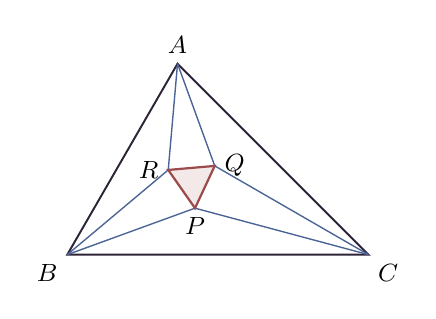
\begin{tikzpicture}[scale=0.85]
			\coordinate (B) at (0,0);
			\coordinate (C) at (4.5,0);
			\coordinate (Btop) at ($(B)+(60:5)$);
			\coordinate (Ctop) at ($(C)+(135:5)$);
			\coordinate (A) at (intersection of B--Btop and C--Ctop);
			
			\coordinate (Br) at ($(B)+(40:4)$);
			\coordinate (Bp) at ($(B)+(20:4)$);
			\coordinate (Cp) at ($(C)+(165:4)$);
			\coordinate (Cq) at ($(C)+(150:4)$);
			\coordinate (Ar) at ($(A)+(265:4)$);
			\coordinate (Aq) at ($(A)+(290:4)$);
			
			\coordinate (R) at (intersection of B--Br and A--Ar);
			\coordinate (P) at (intersection of B--Bp and C--Cp);
			\coordinate (Q) at (intersection of A--Aq and C--Cq);
			
			\draw[line width=0.7pt,morleydark] (A) -- (B) -- (C) -- cycle;
			
			\draw[morleyblue,line width=0.5pt] (A) -- (R);
			\draw[morleyblue,line width=0.5pt] (A) -- (Q);
			\draw[morleyblue,line width=0.5pt] (B) -- (R);
			\draw[morleyblue,line width=0.5pt] (B) -- (P);
			\draw[morleyblue,line width=0.5pt] (C) -- (P);
			\draw[morleyblue,line width=0.5pt] (C) -- (Q);
			
			\fill[morleyred!12] (P) -- (Q) -- (R) -- cycle;
			\draw[morleyred,line width=0.8pt] (P) -- (Q) -- (R) -- cycle;
			
			\node[above,font=\small] at (A) {$A$};
			\node[below left,font=\small] at (B) {$B$};
			\node[below right,font=\small] at (C) {$C$};
			\node[left,font=\small] at (R) {$R$};
			\node[below,font=\small] at (P) {$P$};
			\node[right,font=\small] at (Q) {$Q$};
		\end{tikzpicture}
		\captionof{figure}{Geometric setup for the trigonometric proof.}
		\label{fig:trig}
	\end{minipage}
	
	\vspace{0.5cm} 
	
	\subsection{Computing Intermediary Sides}
	Consider $\Delta BPC$. The angles at $B$ and $C$ generated by the adjacent trisectors are $\beta$ and $\gamma$, respectively. The remaining angle is $m(\angle BPC) = \pi - (\beta + \gamma)$. Applying the Law of Sines to $\Delta BPC$ to find the length of $BP$, we obtain:
	\[ 
	BP = \frac{BC \sin(\gamma)}{\sin(\pi - (\beta + \gamma))} = \frac{2 \sin(3\alpha) \sin(\gamma)}{\sin(\pi/3 + \alpha)} 
	\]
	The denominator simplifies because $\beta + \gamma = \pi/3 - \alpha$, giving $\pi - (\pi/3 - \alpha) = 2\pi/3 + \alpha$. The sine of this angle is identically $\sin(\pi/3 - \alpha)$.
	
	We invoke the trigonometric triple-angle identity $\sin(3\alpha) = 3\sin(\alpha) - 4\sin^3(\alpha)$, which factors as:
	\[
	\sin(3\alpha) = 4 \sin(\alpha) \sin\left(\frac{\pi}{3} + \alpha\right) \sin\left(\frac{\pi}{3} - \alpha\right)
	\]
	Substituting this expansion into our equation for $BP$, the $\sin(\pi/3 - \alpha)$ term in the numerator cancels with the denominator, leaving:
	\[ 
	BP = 8 \sin(\alpha) \sin\left(\frac{\pi}{3} + \alpha\right) \sin(\gamma) 
	\]
	By an identical argument applied to $\Delta BRA$ on the adjacent side of the triangle, we obtain:
	\[ 
	BR = 8 \sin(\gamma) \sin\left(\frac{\pi}{3} + \gamma\right) \sin(\alpha) 
	\]
	
	\subsection{Evaluating the Morley Triangle}
	We now evaluate the side $PR$ of the Morley triangle. Consider $\Delta BPR$, where the central trisected angle is $m(\angle PBR) = \beta$. The Law of Cosines dictates:
	\[ 
	PR^2 = BP^2 + BR^2 - 2(BP)(BR)\cos(\beta) 
	\]
	Substituting our expressions for $BP$ and $BR$, we factor out the common terms $64 \sin^2(\alpha) \sin^2(\gamma)$:
	\begin{multline*} 
		PR^2 = 64 \sin^2(\alpha) \sin^2(\gamma) \bigg[ \sin^2\left(\frac{\pi}{3} + \alpha\right) + \sin^2\left(\frac{\pi}{3} + \gamma\right) 
		- 2 \sin\left(\frac{\pi}{3} + \alpha\right) \sin\left(\frac{\pi}{3} + \gamma\right) \cos(\beta) \bigg] 
	\end{multline*}
	To simplify the bracketed expression, consider an auxiliary triangle inscribed in a unit circle with angles $\frac{\pi}{3}+\alpha$, $\frac{\pi}{3}+\gamma$, and $\beta$ (these sum to $\pi$ since $\alpha+\beta+\gamma = \pi/3$). By the Law of Cosines applied to this auxiliary triangle, the bracketed term represents the square of the chord opposite the angle $\beta$, which is $\sin^2(\beta)$. 
	
	Taking the square root yields:
	\[
	PR = 8 \sin(\alpha) \sin(\beta) \sin(\gamma)
	\]
	Because this distance formula is invariant under permutations of $\alpha, \beta,$ and $\gamma$, analogous calculations for $PQ$ and $QR$ yield identical lengths. Therefore, $\Delta PQR$ is an equilateral triangle.
	
	\section{Proof 2: Complex Numbers}
	
	This algebraic proof, formalized by Letac and discussed by Cundy \cite{cundy}, maps the problem onto the complex unit circle. It relies on points represented as unit-modulus complex numbers (turns).
	
	\subsection{Embedding in the Unit Circle}
	\mbox{} \\ 
	
	\noindent
	\begin{minipage}[t]{0.6\textwidth}
		\vspace{0pt} 
		Let the circumcircle of $\Delta ABC$ be the unit circle $U \subset \mathbb{C}$. We define the affixes of vertices $A, B, C$ as $a^3, b^3, c^3$, where $a, b, c \in U$. The points of trisection of the consecutive arcs $AB, BC, CA$ are given by the intermediate turns $a^2b, ab^2$; $b^2c, bc^2$; $\omega ac^2, \omega^2 a^2c$, where $\omega = e^{2\pi i / 3}$.
	\end{minipage}% 
	\hfill
	\begin{minipage}[t]{0.35\textwidth}
		\vspace{0pt} 
		\centering
		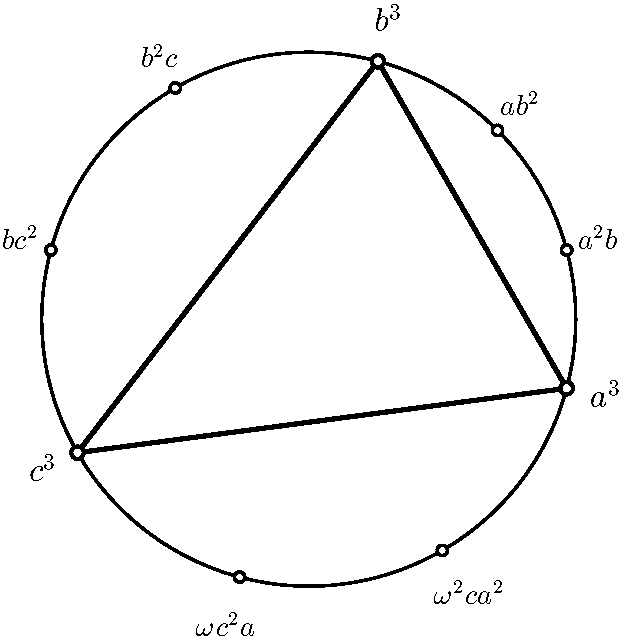
\includegraphics[width=0.6\linewidth]{figure4.pdf}
		\captionof{figure}{Embedding the triangle in the complex unit circle.}
		\label{fig:complex}
	\end{minipage}
	
	\vspace{0.5cm} 
	
	\subsection{Chord Intersections}
	The equation of a line passing through two turns $t, u \in U$ is given by $z + tu z^* = t + u$, where $z^*$ is the complex conjugate. The Morley vertex $x$ is the intersection of two interior trisector chords. Substituting the turns of the trisected arcs yields a simultaneous system:
	\begin{align*}
		x + ab^2c^3 x^* &= ab^2 + c^3 \\
		x + \omega ab^3c^2 x^* &= \omega ac^2 + b^3
	\end{align*}
	Subtracting the second equation from the first and dividing the result by $(c - \omega b)$ yields the conjugate affix of the first Morley vertex:
	\[ 
	a^2b^2c^2 x^* = \omega^2(ab^2 - a^2b) + ac^2 - \omega a^2c + \omega abc 
	\]
	Analogous algebraic expressions are derived for $y^*$ and $z^*$ by cyclic permutation $a \mapsto b \mapsto c \mapsto a$. 
	
	To prove $\Delta xyz$ is equilateral, we verify the condition $x + \omega y + \omega^2 z = 0$. Summing our expressions for $x^*$, $y^*$, and $z^*$ scaled by the appropriate powers of $\omega$ results in the cancellation of the polynomial terms:
	\[ 
	x^* + \omega^2 y^* + \omega z^* = 0 
	\]
	Taking the complex conjugate of this equation yields $x + \omega y + \omega^2 z = 0$. This linear relation shows that the vectors connecting the points $x, y, z$ correspond to rotations by $\pi/3$, indicating they form an equilateral triangle.
	
	\section{Proof 3: Synthetic Proof}
	
	Conway's\cite{conway} proof reverses the theorem: start with an equilateral triangle and build $\triangle ABC$ from 7 pieces.
	
	\subsection{Defining the Seven Pieces}
	\mbox{} \\ 
	
	\noindent
	\begin{minipage}[t]{0.48\textwidth}
		\vspace{0pt} 
		Let $\alpha \!=\! A/3, \beta \!=\! B/3, \gamma \!=\! C/3$, so $\alpha \!+\! \beta \!+\! \gamma \!=\! 60^\circ$.
		Define $\theta^* \!=\! \theta + 60^\circ$ and $\theta^{**} \!=\! \theta + 120^\circ$.
		
		We define the following triangles (their angles sum to $180^\circ$):
		\begin{itemize}
			\item \textbf{1 Central Equilateral:} $0^*, 0^*, 0^*$. Scaled to side-length 1.
			\item \textbf{3 Abutting Triangles:} e.g., $\alpha, \beta^*, \gamma^*$. Scaled so the side opposite $\alpha$ is 1.
			\item \textbf{3 Spoke Triangles:} e.g., $\alpha^{**}, \beta, \gamma$. (Scaling defined in the next subsection).
		\end{itemize}
		These 7 pieces are our building blocks.
	\end{minipage}%
	\hfill
	\begin{minipage}[t]{0.35\textwidth}
		\vspace{0pt} 
		\centering
		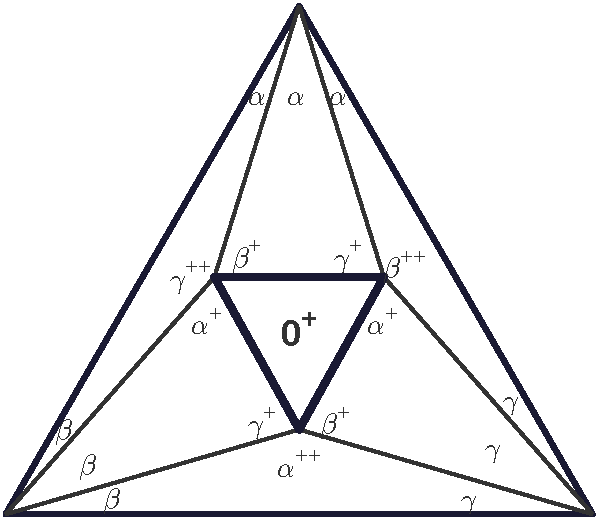
\includegraphics[width=\linewidth]{figure.pdf}
		\captionof{figure}{The seven puzzle pieces for Conway's proof.}
		\label{fig:puzzle}
	\end{minipage}
	
	\vspace{0.5cm} 
	
	\subsection{Sizing the Spoke Triangles}
	\mbox{} \\
	
	\noindent
	\begin{minipage}[t]{0.52\textwidth}
		\vspace{0pt}
		We must guarantee the pieces fit together. Consider the spoke triangle $PB'C'$ with angles $\alpha^{**}$ at $P$, $\beta$ at $B'$, and $\gamma$ at $C'$.
		
		Fix points $Y$ and $Z$ on the line $B'C'$ such that the angles $\angle PYB'$ and $\angle PZC'$ equal $\alpha^*$. 
		
		Because $\angle B'PY = 180^\circ - \beta - \alpha^* = \gamma^*$, the sub-triangle $\triangle B'PY$ has angles $\beta, \alpha^*, \gamma^*$. This makes it strictly similar to our abutting triangle!
		
		We scale the spoke triangle so that $PY = PZ = 1$. Now the side $PY$ perfectly matches the side length 1 of the abutting triangle.
	\end{minipage}%
	\hfill
	\begin{minipage}[t]{0.44\textwidth}
		\vspace{0pt}
		\centering
		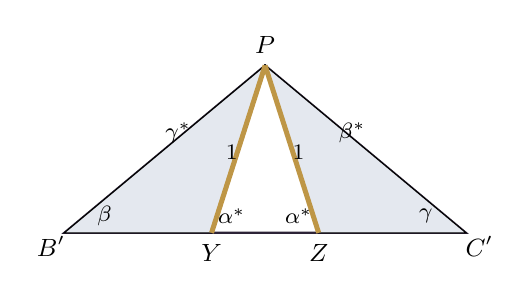
\begin{tikzpicture}[scale=0.85]
			\coordinate (P) at (0, 2.5); \coordinate (Bp) at (-3, 0); \coordinate (Cp) at (3, 0);
			
			\draw[line width=0.8pt, morleydark] (P) -- (Bp) -- (Cp) -- cycle;
			
			\coordinate (Y) at (-0.8, 0); \coordinate (Z) at (0.8, 0);
			
			\draw[fill=morleyblue!15] (P) -- (Bp) -- (Y) -- cycle;
			\draw[fill=morleyblue!15] (P) -- (Cp) -- (Z) -- cycle;
			
			\draw[line width=1.8pt, morleygold] (P) -- (Y);
			\draw[line width=1.8pt, morleygold] (P) -- (Z);
			
			\node[font=\small] at (0, 2.8) {$P$};
			\node[font=\small] at (-3.2, -0.2) {$B'$};
			\node[font=\small] at (3.2, -0.2) {$C'$};
			\node[font=\small] at (-0.8, -0.3) {$Y$};
			\node[font=\small] at (0.8, -0.3) {$Z$};
			
			\node[font=\footnotesize] at (-0.5, 1.2) {$1$}; \node[font=\footnotesize] at (0.5, 1.2) {$1$};
			
			\node[font=\footnotesize] at (-2.4, 0.25) {$\beta$}; \node[font=\footnotesize] at (2.4, 0.25) {$\gamma$};
			\node[font=\footnotesize] at (-0.5, 0.25) {$\alpha^*$}; \node[font=\footnotesize] at (0.5, 0.25) {$\alpha^*$};
			\node[font=\footnotesize] at (-1.3, 1.5) {$\gamma^*$}; \node[font=\footnotesize] at (1.3, 1.5) {$\beta^*$};
		\end{tikzpicture}
		\captionof{figure}{Sizing the spoke triangle to fit abutting triangles.}
		\label{fig:spoke}
	\end{minipage}
	
	\vspace{0.5cm}
	
	\subsection{Assembling the Master Triangle}
	\mbox{} \\
	
	\noindent
	\begin{minipage}[t]{0.52\textwidth}
		\vspace{0pt}
		We attach the three abutting triangles to the central equilateral $\triangle PQR$. Does the spoke triangle fit into the remaining gap at $P$?
		
		The angles meeting at $P$ from the equilateral and abutting triangles are $60^\circ$, $\gamma^*$, and $\beta^*$. Their sum is:
		\[ 60^\circ + (\gamma + 60^\circ) + (\beta + 60^\circ) = 180^\circ + \beta + \gamma \]
		Since $\alpha + \beta + \gamma = 60^\circ$, this is $240^\circ - \alpha$. The remaining gap is $360^\circ - (240^\circ - \alpha) = 120^\circ + \alpha = \alpha^{**}$. This exactly accommodates the spoke triangle $PB'C'$!
		
		By ASA congruence ($\triangle B'PY \cong \triangle BPR$), $B'P = BP$, so $B'$ is precisely the vertex $B$. Assembling all 7 pieces yields a perfect triangle $ABC$. The total angle at $B$ is $\beta \!+\! \beta \!+\! \beta = 3\beta$, proving $BP, BR$ are trisectors!
	\end{minipage}%
	\hfill
	\begin{minipage}[t]{0.35\textwidth}
		\vspace{0pt}
		\centering
		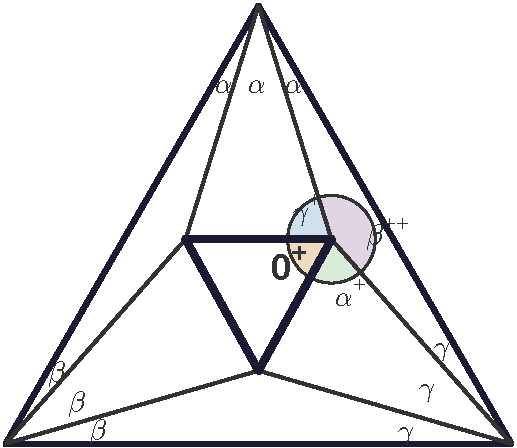
\includegraphics[width=\linewidth]{figure5.pdf}
		\captionof{figure}{Assembling the pieces into the master triangle.}
		\label{fig:assembly}
	\end{minipage}
	
	\section{Proof 4: Group Theory Proof}
	Alain Connes formulated an elegant proof \cite{connes} that bypasses traditional geometric constructions. Instead of managing complex intersecting lines, Connes characterizes Morley's theorem purely as an algebraic property by translating the geometry into the affine group of the complex line.
	
	\subsection{The Affine Framework}
	Let $G$ be the affine group of $\mathbb{C}$. This group acts as our mathematical framework, where an element $g \in G$ takes the form $g(x) = ax + b$. Here, the rotational component is handled by $a \in \mathbb{C}^*$, and the translational shift is handled by $b \in \mathbb{C}$. For any pure rotation ($a \neq 1$), the transformation possesses a unique fixed point where $x$ maps to itself: $\text{fix}(g) = \frac{b}{1-a}$.
	
	\subsection{Encoding the Intersections}
	We can encode the triangle's geometry directly into this framework. Let $g_1, g_2, g_3$ be affine rotations about the vertices $A, B, C$ by angles $2\alpha, 2\beta, 2\gamma$ respectively. The rotational parameters multiply to $a_1 a_2 a_3 = j$, where $j = e^{2\pi i/3}$.
	
	The brilliance of this approach is that the adjacent trisector intersections of the Morley triangle are captured perfectly as the fixed points of the pairwise products of these affine maps: $\alpha = \text{fix}(g_1 g_2)$, $\beta = \text{fix}(g_2 g_3)$, and $\gamma = \text{fix}(g_3 g_1)$.
	
	\subsection{The Equilateral Extraction}
	Because the interior angles of any Euclidean triangle sum to $\pi$, applying all three rotations fully around the triangle results in a net zero rotation and zero translation. Algebraically, the product of the cubes of these transformations is the identity: $g_1^3 g_2^3 g_3^3 = 1$.
	
	This identity forces the translational part of the final equation, $b$, to be exactly zero. By computing this affine product, Connes forces a polynomial expansion that factors beautifully:
	$$b = -j a_1^2 a_2 (a_1 - j)(a_2 - j)(a_3 - j)(\alpha + j\beta + j^2\gamma)$$
	Since $g_1^3 g_2^3 g_3^3 = 1$ makes $b = 0$ a geometric certainty, and the pairwise products are not pure translations (meaning $a_k - j \neq 0$), the final remaining factor must vanish:
	$$\alpha + j\beta + j^2\gamma = 0$$
	This relation is the standard algebraic condition for $\alpha, \beta, \gamma$ to form an equilateral triangle. The geometric intersection has been proven entirely through algebraic factorization.
	
	\section{Proof 5: Circle Geometry}
	
	This proof utilizes inscribed angles and auxiliary circles as formulated by Nancy Walls \cite{walls}.
	
	\subsection{Construction}
	\mbox{} \\ 
	
	\noindent
	\begin{minipage}[t]{0.6\textwidth}
		\vspace{0pt} 
		Start with an equilateral triangle $P_1 P_2 P_3$ and three angles $a_1, a_2, a_3$ such that their sum is $\pi/3$.
		Construct three auxiliary circles $S_i$ ($i=1,2,3$) passing through $P_j, P_k$ such that the chord $P_j P_k$ subtends an angle $a_i$ at the circumference. 
		
		Identify points $Q_i, R_i$ on the boundary of $S_i$ such that the chords $Q_i P_k$ and $P_j R_i$ are equal in length to the base chord $P_j P_k$. Extend the lines $Q_k R_i$ and $R_j Q_i$ until they intersect at the outer vertices $X_i$.
	\end{minipage}% 
	\hfill
	\begin{minipage}[t]{0.35\textwidth}
		\vspace{0pt} 
		\centering
		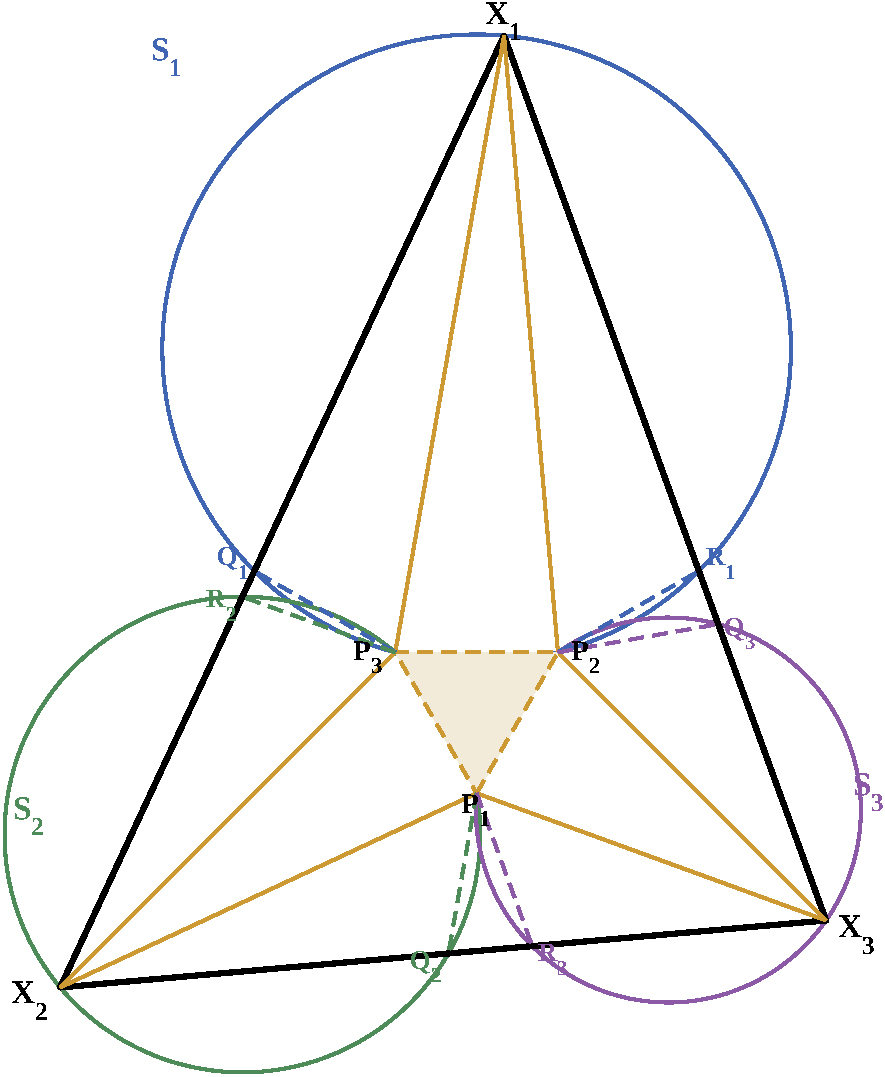
\includegraphics[width=0.6\linewidth]{figure1.pdf}
		\captionof{figure}{Auxiliary circles and pentagon construction.}
		\label{fig:circles}
	\end{minipage}
	
	\vspace{0.5cm} 
	
	\subsection{Angle Chase}
	An angle chase demonstrates that the pentagon $P_j Q_k X_i R_j P_k$ has interior angles summing to $3\pi$. This implies $m(\angle Q_i X_i R_i) = 3a_i$. Because $3a_i$ is the angle subtended at the circumference of $S_i$, the point $X_i$ lies on the circle $S_i$. 
	
	Since the chords are equal in length, the inscribed angles they subtend are equal. Therefore, the lines $X_i P_j$ and $X_i P_k$ trisect the angle $\angle X_i$. Consequently, $X_1 X_2 X_3$ forms the outer triangle similar to $\Delta ABC$, with $P_1 P_2 P_3$ as its inner Morley triangle.
	
	\section{Beyond the Proofs}
	
\subsection{Cardioids and Inversive Geometry}Frank Morley's initial 1899 discovery was deeply connected to algebraic curves, specifically tangent cardioids \cite{morley1933}. Morley demonstrated that if a variable cardioid is tangent to the three extended sides of $\Delta ABC$, the locus of its center consists of nine lines intersecting at 27 points. These 27 points correspond precisely to the intersections of the general (internal and external) trisectors of the triangle. At these specific intersection points, the cardioid is doubly tangent to one of the triangle's sides. Oakley and Baker \cite{oakley} note that Morley's primary focus was actually on these cardioid systems, with the now-famous triangle theorem emerging as a remarkable geometric byproduct.\subsection{Holonomy}The theorem can also be analyzed via differential geometry. Utilizing a method conceptualized by John Smillie and formalized by Peter Doyle \cite{doyle}, one can construct marked similarity triangles (MSTs) around an internal vertex to compute a local invariant known as \textit{holonomy} (the scale factor between a leading edge and a lagging edge). By demonstrating that the product of these local holonomies over a fundamental period equates to $1$ (trivial holonomy), the proof guarantees that these local triangles fit perfectly around the vertex without any angle deficits or overlaps, forming a flat planar geometry. This holonomic invariant serves as the foundational mathematical engine for John Conway's celebrated puzzle-piece construction \cite{conway}.
	
	\vspace{1em}
	\begin{thebibliography}{10}
		
		\bibitem{connes} 
		Connes, A. (1998). A new proof of Morley's theorem. 
		\textit{Publications Math\'ematiques de l'I.H.\'E.S.}, S88, 43--46.
		
		\bibitem{conway} 
		Conway, J. H. (2005). The power of mathematics. 
		In A. F. Blackwell \& D. MacKay (Eds.), \textit{Power} (pp. 16--36). Cambridge University Press.
		
		\bibitem{cundy} 
		Cundy, H. M. (1984). A direct proof of Morley's theorem. 
		\textit{The Mathematical Gazette}, 68(444), 112--119.
		
		\bibitem{doyle}
		Doyle, P., \& Sethi, S. (2018). Conway's doughnuts. 
		arXiv:1804.04024.
		
		\bibitem{morley1900} 
		Morley, F. (1900). On the metric geometry of the plane n-line. 
		\textit{Transactions of the American Mathematical Society}, 1, 97--115.
		
		\bibitem{morley1933}
		Morley, F., \& Morley, F. V. (1933). \textit{Inversive Geometry}. 
		G. Bell and Sons.
		
		\bibitem{newman}
		Newman, D. J. (1996). The Morley Miracle. 
		\textit{The Mathematical Intelligencer}, 18(1), 31--32.
		
		\bibitem{oakley}
		Oakley, C. O., \& Baker, J. C. (1978). The Morley Trisector Theorem. 
		\textit{The American Mathematical Monthly}, 85(9), 737--745.
		
		\bibitem{taylor}
		Taylor, F. G., \& Marr, W. L. (1914). The six trisectors of each of the angles of a triangle. 
		\textit{Proceedings of the Edinburgh Mathematical Society}, 32, 119--131.
		
		\bibitem{walls}
		Walls, N. (1944). An Elementary Proof of Morley's Trisector Theorem. 
		\textit{The Mathematical Gazette}, 28(278), 12--13.
		
	\end{thebibliography}
	
	% ==========================================
	% APPENDIX
	% ==========================================
	\newpage
	\appendix
	
	\section{MATLAB Source Code for Figures}
	The following MATLAB script was developed to accurately compute the coordinates, simulate the geometric relationships, and render the vector figures presented throughout this report.
	
	\begin{lstlisting}[caption={Geometric simulation and plotting script}]
		clear; clc; close all;
		
		%% Figure 1: Alpha/Beta/Gamma Overview
		A1 = [0, 10]; B1 = [-8.66, -5]; C1 = [8.66, -5];     
		D1 = [-2.5, 2]; E1 = [2.5, 2]; F1 = [0, -2.5];      
		figure('Color', 'w'); hold on; axis equal; axis off;
		outerColor = [0.1 0.1 0.2]; auxColor = [0.2 0.2 0.2]; textColor = [0.2 0.2 0.2];
		fontSize = 14;
		plot([B1(1) A1(1) C1(1) B1(1)], [B1(2) A1(2) C1(2) B1(2)], 'Color', outerColor, 'LineWidth', 2.5);
		plot([A1(1) D1(1)], [A1(2) D1(2)], 'Color', auxColor, 'LineWidth', 1.5);
		plot([A1(1) E1(1)], [A1(2) E1(2)], 'Color', auxColor, 'LineWidth', 1.5);
		plot([B1(1) D1(1)], [B1(2) D1(2)], 'Color', auxColor, 'LineWidth', 1.5);
		plot([B1(1) F1(1)], [B1(2) F1(2)], 'Color', auxColor, 'LineWidth', 1.5);
		plot([C1(1) E1(1)], [C1(2) E1(2)], 'Color', auxColor, 'LineWidth', 1.5);
		plot([C1(1) F1(1)], [C1(2) F1(2)], 'Color', auxColor, 'LineWidth', 1.5);
		plot([D1(1) E1(1) F1(1) D1(1)], [D1(2) E1(2) F1(2) D1(2)], 'Color', outerColor, 'LineWidth', 3.5);
		text(-.35, 7.4, '\alpha', 'FontSize', fontSize, 'Color', textColor);
		text(0.9, 7.4, '\alpha', 'FontSize', fontSize, 'Color', textColor);
		text(-1.5, 7.4, '\alpha', 'FontSize', fontSize, 'Color', textColor);
		text(-6.5, -3.5, '\beta', 'FontSize', fontSize, 'Color', textColor);
		text(-5.8, -4.5, '\beta', 'FontSize', fontSize, 'Color', textColor);
		text(-7.2, -2.5, '\beta', 'FontSize', fontSize, 'Color', textColor);
		text(5.5, -3, '\gamma', 'FontSize', fontSize, 'Color', textColor);
		text(4.8, -4.5, '\gamma', 'FontSize', fontSize, 'Color', textColor);
		text(6, -1.6, '\gamma', 'FontSize', fontSize, 'Color', textColor);
		text(-3.8, 2.1, '\gamma^{++}', 'FontSize', fontSize, 'Color', textColor);
		text(2.5, 2.4, '\beta^{++}', 'FontSize', fontSize, 'Color', textColor);
		text(0, -3.5, '\alpha^{++}', 'FontSize', fontSize, 'Color', textColor, 'HorizontalAlignment', 'center');
		text(-3.2, 0.7, '\alpha^+', 'FontSize', fontSize, 'Color', textColor);
		text(-2, 2.7, '\beta^+', 'FontSize', fontSize, 'Color', textColor);
		text(2, 0.7, '\alpha^+', 'FontSize', fontSize, 'Color', textColor);
		text(1, 2.7, '\gamma^+', 'FontSize', fontSize, 'Color', textColor);
		text(-1.5, -2.2, '\gamma^+', 'FontSize', fontSize, 'Color', textColor);
		text(0.6, -2.2, '\beta^+', 'FontSize', fontSize, 'Color', textColor);
		text(0, 0.5, '0^+', 'FontSize', 18, 'FontWeight', 'bold', 'HorizontalAlignment', 'center', 'Color', textColor);
		hold off;
		
		%% Figure 2: The S-Circle Construction
		alpha1 = 15 * pi/180; alpha2 = 20 * pi/180; alpha3 = 25 * pi/180;
		L = 4;
		P1 = [0, -L/sqrt(3)]; P2 = [L/2, L/(2*sqrt(3))]; P3 = [-L/2, L/(2*sqrt(3))];
		[O1, r1, Q1, R1] = buildReverseCircle([0,0], P2, P3, alpha1);
		[O2, r2, Q2, R2] = buildReverseCircle([0,0], P3, P1, alpha2);
		[O3, r3, Q3, R3] = buildReverseCircle([0,0], P1, P2, alpha3);
		X1 = getIntersect(Q1, R2, R1, Q3);
		X2 = getIntersect(Q2, R3, R2, Q1);
		X3 = getIntersect(Q3, R1, R3, Q2);
		figure('Color', 'w', 'Position', [100, 100, 850, 850]); hold on; axis equal; axis off;
		color_S1 = [0.25, 0.40, 0.70]; color_S2 = [0.30, 0.55, 0.35]; color_S3 = [0.55, 0.35, 0.65]; 
		color_lines = [0.80, 0.60, 0.20]; color_fill = [0.95, 0.92, 0.85];
		drawCircle(O1, r1, color_S1); drawCircle(O2, r2, color_S2); drawCircle(O3, r3, color_S3);
		plot([X1(1), X2(1), X3(1), X1(1)], [X1(2), X2(2), X3(2), X1(2)], 'k', 'LineWidth', 2.5);
		patch([P1(1), P2(1), P3(1)], [P1(2), P2(2), P3(2)], color_fill, 'EdgeColor', 'none');
		plot([P1(1), P2(1), P3(1), P1(1)], [P1(2), P2(2), P3(2), P1(2)], '--', 'Color', color_lines, 'LineWidth', 1.5);
		text(X1(1), X1(2) + 0.4, 'X_1', 'FontSize', 16, 'FontWeight', 'bold');
		text(P1(1), P1(2) - 0.4, 'P_1', 'FontSize', 14, 'FontWeight', 'bold');
		hold off;
		
		%% Figure 3: Angular Sectors at Vertex E
		A3 = [0, 10]; B3 = [-8.66, -5]; C3 = [8.66, -5]; E3 = [2.5, 2];
		figure('Color', 'w'); hold on; axis equal; axis off;
		r_arc = 1.5; cx = E3(1); cy = E3(2);
		th_A = atan2(A3(2)-cy, A3(1)-cx); th_D = pi; th_C = atan2(C3(2)-cy, C3(1)-cx); th_F = atan2(-2.5-cy, 0-cx);
		fill([cx, cx + r_arc*cos(linspace(th_A, th_D, 50)), cx], [cy, cy + r_arc*sin(linspace(th_A, th_D, 50)), cy], [0.82, 0.88, 0.93], 'EdgeColor', 'none');
		fill([cx, cx + r_arc*cos(linspace(th_C, th_A, 50)), cx], [cy, cy + r_arc*sin(linspace(th_C, th_A, 50)), cy], [0.88, 0.84, 0.89], 'EdgeColor', 'none');
		plot([B3(1) A3(1) C3(1) B3(1)], [B3(2) A3(2) C3(2) B3(2)], 'Color', [0.1 0.1 0.2], 'LineWidth', 2.5);
		text(1.1, 1.2, '0^+', 'FontSize', 18, 'FontWeight', 'bold', 'Color', textColor);
		hold off;
		
		%% Figure 4: Unit Circle Chord Intersections
		figure('Color', 'w', 'Position', [150, 150, 800, 800]); hold on; axis equal; axis off;
		g_circ = [0.65, 0.65, 0.70]; m_edg = [0.15, 0.12, 0.15]; b_ln = [0.35, 0.45, 0.65];
		p_ln = [0.55, 0.40, 0.60]; o_ln = [0.85, 0.55, 0.25]; i_fll = [0.90, 0.82, 0.82]; i_edg = [0.65, 0.35, 0.35];
		get_pt = @(ang) [cosd(ang), sind(ang)];
		A4 = get_pt(-5); B4 = get_pt(85); C4 = get_pt(205);
		Pp1 = get_pt(50); Pp2 = get_pt(22); Po1 = get_pt(260);
		x_pt = intersectLines(C4, Pp1, B4, Po1);
		y_pt = intersectLines(C4, Pp2, B4, Po1);
		Pb1 = intersectCircle(A4, x_pt);
		Pb2 = intersectCircle(A4, y_pt);
		z_pt = intersectLines(A4, Pb1, C4, Pp2);
		Po2 = intersectCircle(B4, z_pt);
		theta = linspace(0, 360, 300);
		plot(cosd(theta), sind(theta), 'Color', g_circ, 'LineWidth', 1.5);
		fill([x_pt(1), y_pt(1), z_pt(1)], [x_pt(2), y_pt(2), z_pt(2)], i_fll, 'EdgeColor', 'none');
		plot([A4(1), Pb1(1)], [A4(2), Pb1(2)], 'Color', b_ln, 'LineWidth', 1.5);
		plot([A4(1), Pb2(1)], [A4(2), Pb2(2)], 'Color', b_ln, 'LineWidth', 1.5);
		plot([C4(1), Pp1(1)], [C4(2), Pp1(2)], '--', 'Color', p_ln, 'LineWidth', 1.5);
		plot([C4(1), Pp2(1)], [C4(2), Pp2(2)], '--', 'Color', p_ln, 'LineWidth', 1.5);
		plot([B4(1), Po1(1)], [B4(2), Po1(2)], '--', 'Color', o_ln, 'LineWidth', 1.5);
		plot([B4(1), Po2(1)], [B4(2), Po2(2)], '--', 'Color', o_ln, 'LineWidth', 1.5);
		plot([x_pt(1), y_pt(1), z_pt(1), x_pt(1)], [x_pt(2), y_pt(2), z_pt(2), x_pt(2)], 'Color', i_edg, 'LineWidth', 3);
		plot([A4(1), B4(1), C4(1), A4(1)], [A4(2), B4(2), C4(2), A4(2)], 'Color', m_edg, 'LineWidth', 3);
		text(A4(1)+0.07, A4(2)+0.06, '$a^3$', 'Interpreter', 'latex', 'FontSize', 24);
		text(x_pt(1)-0.09, x_pt(2)+0.02, '$x$', 'Interpreter', 'latex', 'FontSize', 18);
		xlim([-1.2 1.2]); ylim([-1.2 1.2]);
		hold off;
		
		%% Figure 5: Complex Turns
		theta_a = -5*pi/180; theta_b = 25*pi/180; theta_c = 70*pi/180;
		a = exp(1i*theta_a); b = exp(1i*theta_b); c = exp(1i*theta_c); w = exp(1i*2*pi/3);
		figure('Color', 'w'); hold on; axis equal; axis off;
		plot(cos(linspace(0, 2*pi, 200)), sin(linspace(0, 2*pi, 200)), 'k', 'LineWidth', 1.2);
		plot(real([a^3, b^3, c^3, a^3]), imag([a^3, b^3, c^3, a^3]), 'k', 'LineWidth', 2);
		text(real(a^3)*1.15, imag(a^3)*1.15, '$a^3$', 'Interpreter', 'latex', 'FontSize', 16, 'Color', 'k');
		hold off;
		
		%% Local Functions
		function [O, r, Q, R] = buildReverseCircle(Pc, A, B, alpha)
		M = (A + B) / 2; AB = B - A; N = [-AB(2), AB(1)]; N = N / norm(N);
		if dot(N, M - Pc) < 0, N = -N; end
		O = M + (norm(AB)/2) * cot(alpha) * N; r = norm(A - O);
		phi_A = atan2(A(2) - O(2), A(1) - O(1)); phi_B = atan2(B(2) - O(2), B(1) - O(1));
		delta = mod(phi_B - phi_A + pi, 2*pi) - pi;
		Q = O + r * [cos(phi_B + delta), sin(phi_B + delta)];
		R = O + r * [cos(phi_A - delta), sin(phi_A - delta)];
		end
		function pt = getIntersect(P1, P2, P3, P4)
		A_mat = [P2(2)-P1(2), P1(1)-P2(1); P4(2)-P3(2), P3(1)-P4(1)];
		b_vec = [A_mat(1,1)*P1(1) + A_mat(1,2)*P1(2); A_mat(2,1)*P3(1) + A_mat(2,2)*P3(2)];
		pt = (A_mat \ b_vec)';
		end
		function drawCircle(O, r, color)
		t = linspace(0, 2*pi, 200); plot(O(1) + r*cos(t), O(2) + r*sin(t), 'Color', color, 'LineWidth', 1.5);
		end
		function P = intersectLines(p1, p2, p3, p4)
		den = (p1(1)-p2(1))*(p3(2)-p4(2)) - (p1(2)-p2(2))*(p3(1)-p4(1));
		P(1) = ((p1(1)*p2(2) - p1(2)*p2(1))*(p3(1)-p4(1)) - (p1(1)-p2(1))*(p3(1)*p4(2) - p3(2)*p4(1))) / den;
		P(2) = ((p1(1)*p2(2) - p1(2)*p2(1))*(p3(2)-p4(2)) - (p1(2)-p2(2))*(p3(1)*p4(2) - p3(2)*p4(1))) / den;
		end
		function P_ext = intersectCircle(p_start, p_through)
		v = p_through - p_start;
		t = -2 * (p_start(1)*v(1) + p_start(2)*v(2)) / (v(1)^2 + v(2)^2);
		P_ext = p_start + t * v;
		end
	\end{lstlisting}
	\newpage
	\section{TikZ Source Code for Diagrams}
	The following TikZ code blocks were used to generate the inline geometric diagrams directly within LaTeX, utilizing the custom color palette defined in the document preamble.
	
	\subsection{Trigonometry Proof Diagram}
	\begin{lstlisting}[language=TeX, caption={TikZ code for the trigonometric geometric setup}]
		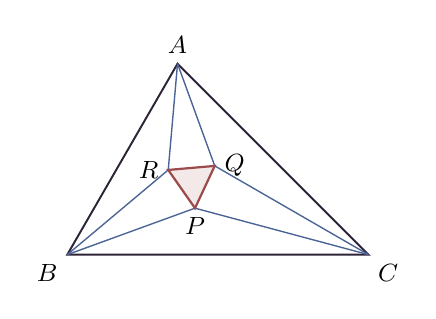
\begin{tikzpicture}[scale=0.85]
			\coordinate (B) at (0,0);
			\coordinate (C) at (4.5,0);
			\coordinate (Btop) at ($(B)+(60:5)$);
			\coordinate (Ctop) at ($(C)+(135:5)$);
			\coordinate (A) at (intersection of B--Btop and C--Ctop);
			
			\coordinate (Br) at ($(B)+(40:4)$);
			\coordinate (Bp) at ($(B)+(20:4)$);
			\coordinate (Cp) at ($(C)+(165:4)$);
			\coordinate (Cq) at ($(C)+(150:4)$);
			\coordinate (Ar) at ($(A)+(265:4)$);
			\coordinate (Aq) at ($(A)+(290:4)$);
			
			\coordinate (R) at (intersection of B--Br and A--Ar);
			\coordinate (P) at (intersection of B--Bp and C--Cp);
			\coordinate (Q) at (intersection of A--Aq and C--Cq);
			
			\draw[line width=0.7pt,morleydark] (A) -- (B) -- (C) -- cycle;
			
			\draw[morleyblue,line width=0.5pt] (A) -- (R);
			\draw[morleyblue,line width=0.5pt] (A) -- (Q);
			\draw[morleyblue,line width=0.5pt] (B) -- (R);
			\draw[morleyblue,line width=0.5pt] (B) -- (P);
			\draw[morleyblue,line width=0.5pt] (C) -- (P);
			\draw[morleyblue,line width=0.5pt] (C) -- (Q);
			
			\fill[morleyred!12] (P) -- (Q) -- (R) -- cycle;
			\draw[morleyred,line width=0.8pt] (P) -- (Q) -- (R) -- cycle;
			
			\node[above,font=\small] at (A) {$A$};
			\node[below left,font=\small] at (B) {$B$};
			\node[below right,font=\small] at (C) {$C$};
			\node[left,font=\small] at (R) {$R$};
			\node[below,font=\small] at (P) {$P$};
			\node[right,font=\small] at (Q) {$Q$};
		\end{tikzpicture}
	\end{lstlisting}
	
	\subsection{Spoke Triangle Diagram}
	\begin{lstlisting}[language=TeX, caption={TikZ code for the synthetic spoke triangle setup}]
		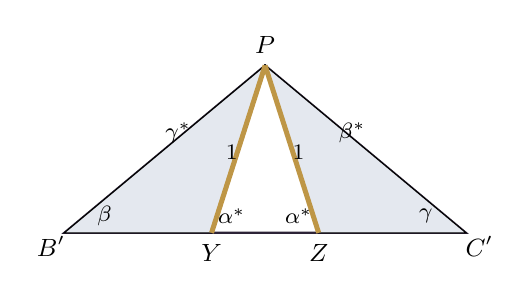
\begin{tikzpicture}[scale=0.85]
			\coordinate (P) at (0, 2.5); 
			\coordinate (Bp) at (-3, 0); 
			\coordinate (Cp) at (3, 0);
			
			\draw[line width=0.8pt, morleydark] (P) -- (Bp) -- (Cp) -- cycle;
			
			\coordinate (Y) at (-0.8, 0); 
			\coordinate (Z) at (0.8, 0);
			
			\draw[fill=morleyblue!15] (P) -- (Bp) -- (Y) -- cycle;
			\draw[fill=morleyblue!15] (P) -- (Cp) -- (Z) -- cycle;
			
			\draw[line width=1.8pt, morleygold] (P) -- (Y);
			\draw[line width=1.8pt, morleygold] (P) -- (Z);
			
			\node[font=\small] at (0, 2.8) {$P$};
			\node[font=\small] at (-3.2, -0.2) {$B'$};
			\node[font=\small] at (3.2, -0.2) {$C'$};
			\node[font=\small] at (-0.8, -0.3) {$Y$};
			\node[font=\small] at (0.8, -0.3) {$Z$};
			
			\node[font=\footnotesize] at (-0.5, 1.2) {$1$}; \node[font=\footnotesize] at (0.5, 1.2) {$1$};
			
			\node[font=\footnotesize] at (-2.4, 0.25) {$\beta$}; \node[font=\footnotesize] at (2.4, 0.25) {$\gamma$};
			\node[font=\footnotesize] at (-0.5, 0.25) {$\alpha^*$}; \node[font=\footnotesize] at (0.5, 0.25) {$\alpha^*$};
			\node[font=\footnotesize] at (-1.3, 1.5) {$\gamma^*$}; \node[font=\footnotesize] at (1.3, 1.5) {$\beta^*$};
		\end{tikzpicture}
	\end{lstlisting}
	
\end{document}